
% to switch between single and double column mode
\documentclass[11pt,twocolumn]{article}
%\documentclass[11pt]{article}

\usepackage{fullpage}
\usepackage{subfigure,indentfirst}
% for url
\usepackage{hyperref}
% for underlined text
\usepackage[normalem]{ulem}
% for including pdf figures
\usepackage{graphicx}

\newenvironment{my_enumerate}{
  \begin{enumerate}
    \setlength{\itemsep}{1pt} 
      \setlength{\parskip}{0pt}
\setlength{\parsep}{0pt}}{\end{enumerate}
}

\newenvironment{my_itemize}{
  \begin{itemize}
    \setlength{\itemsep}{1pt}
      \setlength{\parskip}{0pt}
\setlength{\parsep}{0pt}}{\end{itemize}
}

% this starts the document
\begin{document}

\title{CS87 Project Report: 
Parallelizing Neural Network Training using MPI}

\author{Owen Webb and George Briggs \\
Computer Science Department, Swarthmore College, Swarthmore, PA  19081}

\maketitle

\begin{abstract}

Using the Message Passing Library, this paper will show an approach to parallelizing the training process for a neural network. The model being used will allocate each processor an equal chunk of the data and an exact copy of the neural network, known as Pattern Parallel Training~\cite{dahl:NNCluster}. Each processor will begin training in parallel using their chunk of data. After each iteration, the processors will share their edge weights with each other and compute an average weight for each edge using a reduction tree. Using this parallelization technique, we saw speed up during the training process and even an increase in the accuracy of the network for certain numbers of processors. Training time is often considered the primary limiting factor of neural networks so decreasing training time without sacrificing any accuracy is a significant result. Finally, we will explore the trade-offs in relationships between accuracy and training time, accuracy and number of processors, and training time and number of processors.

\end{abstract}


\section {Introduction} 


% The introduction is the big picture of your work: what, why, and how. It
% includes a definition of the problem you are solving, a high-level description
% of your solution including any novel techniques and results you provide, and a
% summary of the main results of your paper. In addition, motivates the problem
% you are solving (why should a reader find your work important), and describes
% your contribution to the area (this may not be applicable to your project).
% The first paragraph of the introduction should contain all of this information
% in a very high-level. Subsequent paragraphs should discuss in more detail the
% problem you are solving, your solution, and your results and conclusions.

In this paper, the Message Passing Interface library (MPI) will be used to parallelize a neural network with a end goal of speeding up the training time on a generic computing cluster. Long training times is a significant problem facing neural networks, but this can be solved by utilizing data and model parallelism.

Neural networks are a subset of deep learning algorithms that, mimicking the design of neurons in the human brain, are able to model complex patterns in data sets using many hidden layers and non-linear activation functions. They are great in classification problems and regression problems alike. Recently, they have been gaining a lot of popularity due to advances in computer hardware and due to their high levels of accuracy, especially when trained with huge amount of data. They have been at the core of many recent technological advances including image recognition, speech synthesis systems, navigation systems, algorithms of industrial robots, and unmanned vehicles. 
However, while there are certainly many positive qualities of neural networks, these positives come at a cost. In order to achieve these high levels of accuracy and utilize such large amounts of data, neural networks can often require large amounts of time to complete training. The amount of use cases that neural networks currently have is greatly diminished by their long training times. This is why we believe implementing a neural network in parallel to speed up the training process could be very useful, as it addresses one of the primary critiques of a very successful algorithm. 

The goal of this paper is to implement a neural network in parallel to decrease the amount of time required to train while maintaining a similar accuracy to the sequential implementation. Our solution will utilize the Message Passing Interface, MPI\cite{MPI}, library to distribute work and communicate across processors in Swarthmore's Computer Science Network. We start with a sequential implementation of a neural network written in C++ as many of the Machine Learning packages are significantly abstracted. We needed to avoid the abstraction present in these libraries because the areas we wish to parallelize were abstracted away, so the sequential implementation we are utilizing is built from scratch.

Our solution is to distribute data across processors then have the processors reconvene after each iteration. We begin by loading in the data on all processors and  each processor is designated an equal section of the data which is based on its rank. Then in parallel, each processor is given a random set of weights and begins its training process in the same way as the sequential implementation. After the end of an iteration, using a reduction tree (MPI\textunderscore Allreduce function), each processor is given a new set of weights which corresponds to the sum of the weights from each of the processors. Then each processor loops through their weights and divides each summed value by the number of processors to compute an average set of weights. Now, all processors have an identical set of weights when they begin their next iteration of training and this process repeats each iteration. 

There were a number of successful results regarding the speedup and accuracy of our solution. First, increasing the number of processors led to a speed up in training time of the model by a significant rate. For instance, using 2 processors the total training time was 53.6$\%$ faster, using 4 processors the training time was 191.2$\%$ faster, using 8 processors the training time was 227.4$\%$ faster, using 16 processors the training time was 514$\%$ faster, using 32 processors the training time was 1,089$\%$ faster, and finally using 64 processors the training time was 2,174$\%$ faster. In terms of accuracy, not only did the model test at a comparable accuracy to the sequential, but it reported an even higher amount of accuracy for experiments run with 2 and 4 processors. While the sequential model across 3 tests averaged an accuracy of 91.83$\%$, the tests with 2 processors averaged 94.52$\%$ and the tests with 4 processors averaged 95.00$\%$. These increases in accuracy are likely due to a decrease in the amount of over-fitting present in the model which will discuss more in section \ref{results}. The tests with 8, 16, 32, and 64 processors still had relatively high accuracy across tests with averages of 89.07$\%$, 88.71$\%$, 86.09$\%$, and 83.99$\%$ respectively.

Based on the results, we can confidently conclude that the parallel model is capable of speeding up the training process by a significant amount. We also argue that when using 2 or 4 processors to train, the model is at least as accurate as the sequential implementation. We also identify trends in accuracy as it relates to the amount of processors present in the training process. We see a slight increase in the accuracy when the number of processors is low and the neural network is resistant to over-fitting. After the number of processors start increasing more dramatically, the data is stretched too thin across processors and the model is not able to improve upon itself enough in 30 epochs to maintain a high level of accuracy.

The remaining part of the paper is as follows, Section \ref{relwork} will describe related work that has been done previously. Section \ref{soln} will establish the approach that we took to solve this problem. Section \ref{results} as said previously will walk through how the experiments were formed and what they achieved. Section \ref{conc} will touch on what was found after these experiments and how research should extend from here. Section \ref{meta} will establish some of the difficulties faced in this project. 

\section {Related Work}\label{relwork}
% This is an essential part of a research paper; discussing related work is a
% good way to put your work in context with other similar work, and to provide a
% way for you to compare/ contrast your work to other's work.  You should use
% feedback on the annotated bibliography from your project proposal to structure
% this section; it should be written as a re-write of your annotated bibliography
% in a single Related Work section.

With Neural Networks gaining popularity in the computer science field, lots of research has been done to improve them and the training time cost they incur. Multiple approaches to a reduction in training time have been explored. One such approach came from a study performed by  Shallue~\cite{Shallue:NNTraining}, who took the approach of data parallelization. Rather than parallelizing their neural network model, they parallelized their data by distributed the training examples across different processors to compute ‘gradient updates’, then aggregated these updates locally. The primary variable that Shallue tuned for was batch size. Their goal was to see if they could keep increases their batch size without increasing the training time of the model.

In Shallue, Lee, etc \cite{Shallue:NNTraining} show that recent advances in hardware have greatly increased the training ability of neural networks by enabling larger models to be trained on even larger data sets then they ever have before. However, the bottleneck of neural networks remains as time, which both limits their performance and the amount of potential use-cases that they have. This is the motivation behind the attempt to parallelize and increase the speed of the training process. The method of parallelization this paper implemented was data parallelism, which distributed the training examples across different processors to compute `gradient updates’, or higher order derivative information, then aggregates these updates locally. In order to test the performance implications of this parallelization technique, they increased the batch size and measured the effect on training time, by counting the steps required to reach a defined goal. In each experiment, the authors alter the training algorithm, the data set, and model in order to identify any other sources of optimization.

One of the benefits found of data parallelization is its ease of implementation. Contrary to model parallelism which may depend on model size and structure, it can be done on any neural network architecture. An interesting takeaway from this paper was their disagreement with the existing research at the time. In particular, Shallue, etc found no evidence that performance decreases with increased batch sizes, rather that optimization algorithms may allow perfect scaling across many models and data sets. However, increasing batch size cannot be done so blindly or it will inhibit performance. Due to the extra work required to optimize this data parallelism, the authors suggest that large scale systems should consider all types of parallelism at their disposal. A potential implication of this research on our work, is that we may now consider optimizing other aspects of the neural network. 

Dahl, McAvinney and Newhall \cite{dahl:NNCluster} present an alternative for training neural networks on a cluster of workstations. While other similar works have been presented, this work specifically notes that they are trying to limit the amount of communication between processors because on a cluster of workstations the communication cost is just too great. To solve this problem, they present Pattern Parallel Training (PPT). PPT accomplishes this by duplicating the full neural network on each node in the cluster, so that individual nodes are not required to send too much information via MPI to each other during a training session as shown in Figure \ref{PPT}. 
\begin{figure}[t]
    \centerline{
        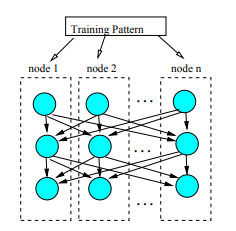
\includegraphics[height=2in]{NPT.png}
    }
    \caption{
        \label{NPT}  Network Parallel Training.
        {\em From Dahl, McAvinney, Newhall \cite{dahl:NNCluster}, a full copy of the network is duplicated on each processor, each processing a portion of the data.}
    }
\end{figure}
\begin{figure}[t]
    \centerline{
        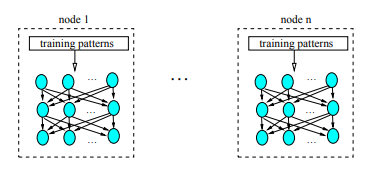
\includegraphics[height=1.5in]{PPT.png}
    }
    \caption{
        \label{PPT}  Pattern Parallel Training. {\em From Dahl, McAvinney, Newhall \cite{dahl:NNCluster}, nodes of a single neural network are split up amongst the processors and updates must be shared every iteration.}
    }
\end{figure}
This improves the overhead cost over most of the previous research that was proposed, Network Parallel Training (NPT). In NPT, nodes of an Artificial Neural Network (ANN) are spread across processors in a cluster as shown in Figure \ref{NPT}. NPT is more appropriate for use when the system is specially designed for a use case. The system can then be built to limit communication costs between nodes, but on a normal workstation system, this collapses due to these costs. PPT also explains how there are certain consistencies that must occur throughout the process such as ensuring at each step the ANNs are identical. They saw a significant speed up for their results which for 8 processors, improved their training time by 10.6 times. The work done in Dahl is the basic apporach that we were looking to accomplish in our solution, but in Section \ref{soln}, we show how this approach can be improved to limit the communication between processors. 

Iandola, Forrest, et al \cite{iandola2016firecaffe} explore the training of a deep neural network on a cluster system with a reduction tree. Because of the need for a reduction in Deep Neural Network (DNN) training time, this paper looks at the development of a new system, FireCaffe, that incorporates a couple of main features that make it unique. First, it establishes that it will be built using a custom cluster of NVIDIA gpus connected via infiniband, which is quicker than ethernet. This helps reduce communication costs in their implementation. For this high bandwidth, low latency model, they use the Titan supercomputer at Oak Ridge Leadership Computing Facility. In addition to the hardware, they have optimized the neural network to achieve minimum communication costs by choosing data parallelism and only communicating when workers are exchanging weight gradients during backpropagation. The last main optimization Iandola, Forrest, et al made was using a reduction tree to compute the weights at each step rather than a parameter server. The process was able to sum the weights from each server in significantly less time compared to parameter server implementation mentioned by Dahl \cite{dahl:NNCluster}. Figure \ref{ParamvsReduc} shows the difference between a parameter server and a reduction tree as drawn by Iandola, Forrest, et al \cite{iandola2016firecaffe}. Training the neural network on ImageNet-1k, which contains over 1 million images, they saw a speedup of over 39x on 128 NVIDIA gpus. This paper differs from the approach described in Section \ref{soln} because in the given experiments, there were not resources to create this custom designed system in the Swarthmore Computer Science network. 

\begin{figure}[t]
    \centerline{
        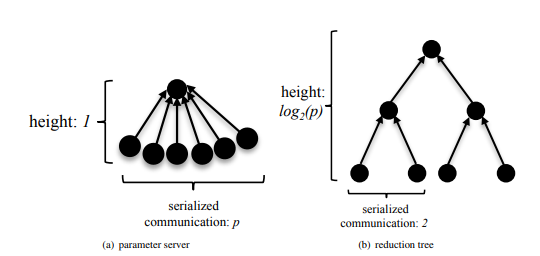
\includegraphics[height=1.65in]{parmservsredtree.png}
    }
    \caption{
        \label{ParamvsReduc}  Parameter Server vs Reduction Tree.
        {\em From Iandola, Forrest, et al \cite{iandola2016firecaffe}, rather than using serialized communication, the Firecaffe system uses a reduction tree to limit serial time.} 
    }
\end{figure}

One very interesting implementation built by Uber Technologies was Horovod.ai which is seen in Sergeev, etc ~\cite{Horovod:journals/corr/abs-1802-05799}. Horovod is a library to run Tenserflow, a popular machine learning framework developed by Google, over a distributed system. This is an abstracted implementation that we are modeling as it is built using MPI on a cluster. The command line resembled MPI as it requires a hostfile, and the number of processors, GPUs in this case, and the file to run. Using this approach would have simplified the project significantly, but also would have been too simple as this was a course project on parallelism.

\section {Solution}\label{soln}
One of the reasons why training a neural network can take so long is it has to forward and backward propagate large amounts of data every iteration of every epoch. For example, in our network which contains 30 epochs and contains roughly 280 iterations for each epoch, we propagating data 8,400 times in our training process which is a significant amount of work. To speed up this process, we will look at making this training occur in parallel so we are not waiting for each training batch to finish before beginning to train the next batch.


\subsection{Materials}

The data set chosen for this project is the industry standard ``Hello World!" for computer vision. The MNST handwritten digit data set is known to be a clean introductory data set that allows users to focus on creating the machine learning model rather than cleaning data. Example digits are shown in Figure \ref{MNIST}. For this reason, we decided from the beginning that we wanted to use this set.

\begin{figure}[t]
    \centerline{
        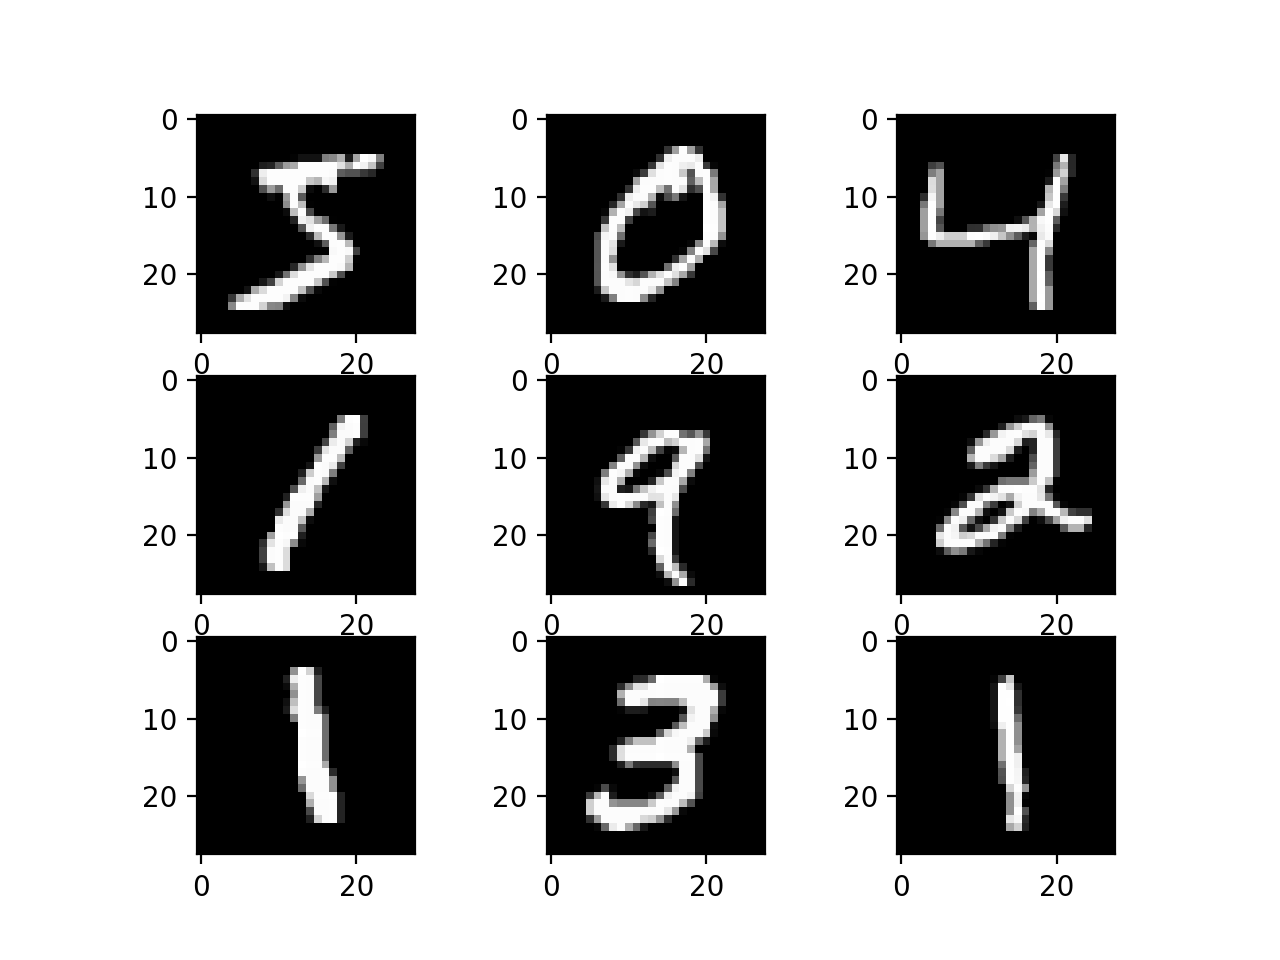
\includegraphics[height=2in]{MNIST.png}
    }
    \caption{\label{MNIST}Example Data {\em MNIST Handwritten Digit Data for a few digits}}
\end{figure}

The first step in implementing the parallel model was to implement a sequential implementation. In the parallel implementation, we need access to the values of weights in the neural network in the middle of the training process so we cannot use a machine learning library that will abstract away the ability to access these values. This is why we began with a sequential neural network built from scratch by \href{https://github.com/tharrington923/neuralnet_handwritten_digit_recognition}{tharrington923}. We will then use the Message Passing Interface (MPI) library as our tool to distribute work across the Swarthmore College Computer Science Network. MPI is a parallel programming communications protocol that is designed for computers that are connected by a network, which is why it is ideal for our purposes.  

\subsection{Splitting Data}
In our parallel model, we will load in the entire data set on each processor. The reason we decided to load in data on all of our processors rather than load in the data on a single processor and distribute the data, is because the loading process occurs in parallel so it should take and equal amount of time to load in on every processor as it would to load in on an individual one and send it to the others. The data is divided up by allocating an equal section of the data to each processor. Processors calculate what section of the data is theirs by using their specific rank. More specifically, they calculate a \emph{size} variable which is equal to the amount of data divided by the number of processes. Then they save the data from the index \emph{size} * \emph{rank} to the index (\emph{size} * \emph{rank}) + \emph{size}.

Now that every processor has an equal amount of data we do not alter our parameters, so we still use the same batch size as long as our processor's subset of data is larger than the specified batch size. Then each processor begins its training the same as the sequential implementation, however, they are now training in parallel.

\subsection{Formatting Data}

Since the data is split up and each processor is trained in parallel, we now have a different neural network on each processor that is the result of one iteration of training, each on a different batch of data. Following the completion of one iteration of training, the next step in the solution is to communicate between processors. 

The goal in this stage is to replace every processor's list of weights with a list of weights that corresponds to an average of all the processor's list of weights. For example, at the end of an iteration of a very simple network running with 2 processors, if one processor has $w_1 = 5$ and $w_2 = 12$ and the other processor has $w_1 = 7$ and $w_2 = 14$, both processors would communicate their weights, compute an average, and replace their set of weights to become $w_1 = 6$ and $w_2 = 11$. They would then start the next iteration with this updated set of weights. 

When communicating weights between processors, the data type of the weights must be altered in order to accommodate MPI's communication methods. This is because our weights are stored in a 3-dimensional C++ vector of doubles, each dimension corresponding to a layer in the neural network. The MPI library does not recognize this data type, so we created a function, \emph{convertToArray}, which loops through the 3-dimensional vector and saves its values into a 1-dimensional C-style array, which is compatible with the MPI library. We also create a very similar function, \emph{convertFromArray} that given a 1-dimensional C-style array, updates the values of our 3-dimensional global weights vector by indexing through the array in the same way it was indexed in during \emph{convertToArray}.

\subsection{Communicating Between Processors}
\subsubsection{Parameter Server}

Now that we have a C-style array, we can utilize MPI's communication method. However, there are many possible ways to communicate the weights and compute an average. This first method that was considered was using a parameter server, as Dahl, McAvinney, Newhall\cite{dahl:NNCluster} used. In this method, a single processor, rank 0, would not be given data to train but would be waiting to receive data from the other processors. Every processor besides rank 0, would train using Pattern Parallel Training shown in Figure \ref{PPT}, then call the \emph{convertToArray} function to create the C-style array of weights and send it to rank 0. Rank 0 first creates an empty local array that is the same size as an array of weights. Then in a for loop, using MPI\textunderscore Receive, rank 0 collects the array of weights from every processor and adds the values from each index to the corresponding index in its local array. After this process is complete, rank 0 has a single local array where every element is the sum of every processor's corresponding weight value. It then loops through the local array dividing each element by $(processors-1)$ so the array becomes an average of the weights. Finally, using an MPI\textunderscore Broadcast, rank 0 sends the averaged array to each of the other processors who then call \emph{convertFromArray} and now can start the next training iteration with their updated identical weights.

\subsubsection{Reduction Tree}
While we initially planned on implementing the parallel model using this method, we recognized that this method requires large amounts of communication, an extra processor to serve as the parameter server, and the averaged weights array is computed sequentially. This most likely would become the bottleneck of our parallel model, so we identified an alternative method utilized by Iandola, Forrest, et al \cite{iandola2016firecaffe}. In this method, rather than using a parameter server to calculate the average weight values, we use a reduction tree as seen in \ref{ParamvsReduc}. A reduction tree takes values from each processor and splits them into groups of two. Each pair makes a computation (in our case this computation will be a sum) and creates a single new value based on this computation. Then another level of pairs are created using the resulting values and this process continues until we are left with one single value. This method is better then the previous for several reasons; it does not require a extra processor to serve as a parameter server, it requires less communication, and the averaged array is computed in parallel. All in all, using a reduction tree is faster and more efficient than a parameter server.

Implementing a reduction tree is a relatively simple process that is very similar to the parameter server. The first step is to call the \emph{convertToArray} function so that each processor has a local C-style array of their weights. We can then implement a reduction tree by using MPI's MPI\textunderscore Allreduce function. Using this function, we can define our operation as SUM and MPI will take each processor's weights array and broadcast back a weights array which contains the sum of every weights. Then in parallel, each processor loops through their new sum array and divides each element by the number of processors, similar to the parameter server method. Finally, each processor can call \emph{convertFromArray} to update their local weights vector and continue on to the next training iteration with the same set of weights as the other processors. 



\section {Results}\label{results}
\subsection{Experiments}

The experiments run were used to analyze two dependent variables, accuracy and training time, and how they are effected by the independent variable, the number of processors. In neural network training, training time and accuracy are the two variables that are analyzed as training time is a bottleneck for most applications. There are cases where the trade off between accuracy and training time would be acceptable. Two sets of experiments are used to create comparisons between these values and draw a conclusion as to the cutoffs.

The first set of experiments ran with solely testing our neural network at the end of training. The goal with these experiments was to create two relationships, one between accuracy and number of processors, then one between training time and number of processors. To do this, each neural network will be trained using the command below, where N is the number of processors. 

\

\verb|mpirun -np N ./neuralnetparallel|

\

For experiment 1, the number processors, N above, will vary from 2 to 64 increasing by a factor of 2 each iteration. This order of vertices allows for training time to decrease significantly after each iteration due to the fact that the outcome is proportional to it. 

The second set of experiments pertain to the accuracy as the neural network trains for each epoch, rather than the amount of time it takes to train and the final accuracy. The experiment will test the accuracy of the neural network at the end of each epoch, to determine how quickly the neural network ``learns". For these experiments, the number of processors, N, will remain the same as the previous experiments. The number of epochs, 30, also remains the same. The difference is the duration will take longer as the duration includes the timing of the testing. The goal of this experiment is to get an insight into how the different number of processors take to level out around the accuracy that they will end up at after 30 Epochs. 

For both experiments in order to offset for any outliers, each experiment will be run 3 times and averaged out so that the most accurate values are achieved. Both experiments used a hostfile that consisted of only the CS87 computers to limit the amount of traffic during testing. The goal of using these computers was to see how the model would perform over ethernet and not infiniband as Iandola, Forrest, et al \cite{iandola2016firecaffe} used.

The reasoning for going not using more than 64 processors in the experiments, was that for this specific data set, the number of batches per processor became too small which did not allow for accurate enough testing as it was training on too little of the data at one time. 


\subsection{Experiment 1} \label{impleres}

\begin{table*}
\begin{center}
\begin{tabular}{|c|c|c|c|}
\hline
\multicolumn{1}{|c|}{Processors}  &\multicolumn{1}{c|}{Duration} &\multicolumn{1}{c|}{Accuracy} &\multicolumn{1}{c|}{Speedup} \\
\hline
2 & 1615.95 & 94.52\% & 1.536 \\
4 & 852.11 & 95.00\% & 2.912\\
8 & 757.89 & 89.07\% & 3.274\\
16 & 404.13 & 88.71\% & 6.140\\
32 & 208.94 & 85.09\% & 11.876\\
64 & 109.12 & 83.99\% & 22.741\\

\hline
\end{tabular}
\caption{\label{exp1res} Experiment 1 Results
  {\em For each number of processors define the duration it took to run 30 Epochs, the accuracy it achieved over those 30 epochs, and the speedup compared 1 processor}}
\end{center}
\end{table*}

Using the implementation described in Section \ref{soln}, the best speedup without sacrificing accuracy, which was the goal, was when we ran using 4 processors. The speedup achieved was 2.912 at an accuracy of 95\%. Looking at Figure \ref{AccvsProcs}, we can safely determine that the number of processors that have the best accuracy is at 4. Also, looking at Figure \ref{AccvsDur}, the accuracy spikes for a training time that coordinates to 4 processors when run for 30 Epochs. From Figure \ref{DurrvsProc}, the most negative derivative comes between 2 processors and 4 processors meaning that for no loss in accuracy, the neural network improves it's time relative to the previous value. As shown in Table \ref{exp1res}, while 64 processors obtains by far the largest speedup relative to 1 processor, there is a 12\% decrease in accuracy for this speedup. For some, this trade-off might be worth it if accuracy is not as important as having a quick speedup. For others, 4 processors might be necessary because they need the highest accuracy the neural network can get. For this experiment, we define the overall ``best" result as the largest drop in duration compared to the sequential while holding the at least the same accuracy for these 30 Epochs. From Table \ref{exp1res}, 4 processors comes out to be the best. 


    
\begin{figure}[t]
    \centerline{
        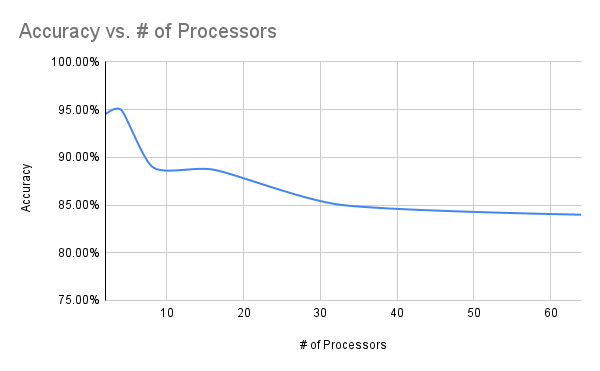
\includegraphics[height=2in]{Accuracy vs. num of Processors.png}
    }
    \caption{\label{AccvsProcs}Experiment 1 Part A {\em The average accuracy after training for 30 Epochs 3 separate times for $2$,$4$,$8$,$16$,$32$,$64$ processors.}}
\end{figure}

\begin{figure}[t]
    \centerline{
        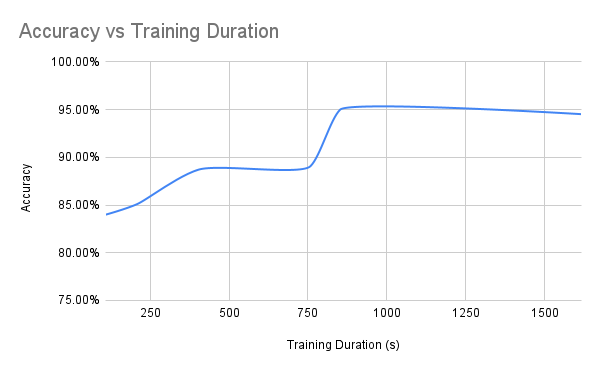
\includegraphics[height=2in]{Accuracy vs Training Duration.png}
    }
    \caption{\label{AccvsDur}  Experiment 1 Part B {\em The accuracy result based on the training duration with an underlying variable of the number of processors. Always run for 30 epochs, training duration depends on the number of processors.}
    }
\end{figure}

\begin{figure}[t]
    \centerline{
        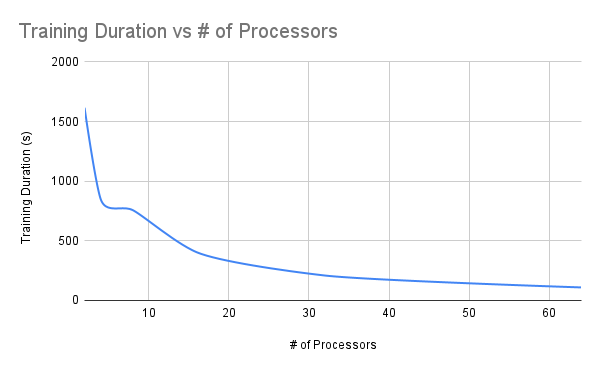
\includegraphics[height=2in]{Training Duration vs num of Processors.png}
    }
    \caption{
        \label{DurrvsProc}  Experiment 1 Part C {\em For running 30 Epochs on varying number of processors, the time duration clearly decreases.}
    }
\end{figure}


\begin{figure*}
    \centering
    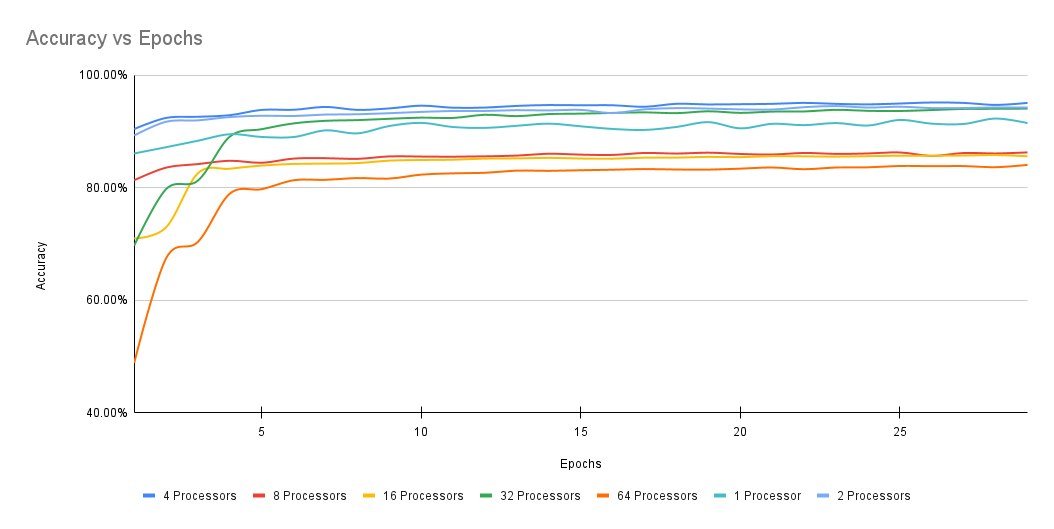
\includegraphics[width=\textwidth,height=3in]{Accuracy vs Epochs.png}
    \caption{\label{accvsepochs} The accuracy vs the number of epochs 
    {\em The accuracy after each epoch is complete for each of the number of processors}
    }
\end{figure*}

 To compare with the sequential neural network, which received an average accuracy over 3 trials of 91.83\% over 30 epochs. The 30 epochs of training time took a total of 2481.36 seconds, equivalent to 41 minutes and 21 seconds. The accuracy we achieved with 4 processors averaged over 3 iterations to 95.00\% with a duration of 852.11 seconds, or 14 minutes and 13 seconds. The speedup of 2.912 was very significant as this actually increased the accuracy of our model which was desired.

\subsection{Experiment 2}

The results for experiment 2 are displayed in Figure \ref{accvsepochs} which shows the accuracy that is achieved after each epoch when testing is done every epoch. This was done to provide a visual to show that after 10 Epochs, the accuracy does not increase significantly for any number of processors. This implies that the accuracy will level out over the course of epochs.

After experiment 1 was run, we hypothesized that maybe the number of epochs, 30, was too small for the greater number of processors to achieve the same accuracy as the smaller number of processors. Because each number of processors levels out at what seems to be a final accuracy, it can be inferred that expanding the number of epochs will not help the accuracy further. 


\section{Conclusions and Future Directions}\label{conc} 


The results from experiment 1 and 2 not only support the goal of creating a parallel neural network that keeps the accuracy the same as the sequential while decreasing the duration of training significantly, but also shows improvement in the training accuracy. Overall, the results were better than we had anticipated at the start of this project. Our original goal was to increase the speed of our training process without sacrificing our accuracy. We are able to achieve significant speedup and not only without decreasing accuracy but likely increasing it. There are several future directions that could be taken to either increase the validity or potentially accuracy of our model. 

To increase the validity and robustness of our model, we would want to try our implementation with different data sets. This could help show the generalizability of our model by proving it is not implemented specifically for this data set. Secondly, one way to potentially increase our accuracy is by tuning for batch size as done by Shallue, Lee, et al\cite{Shallue:NNTraining}. Currently, the batch size is a parameter in the training call, so regardless of how much data is in each processor, they will use the same batch size. We could look at making our batch size a function of the amount of data in each rank rather than leaving it as a parameter in the training function. Another possible way to increase accuracy could be to utilize a weighted average rather than a simple average. If we multiply our weights by their associated network's accuracy, the higher accuracy models will have more impact during the reduction tree. However, this would likely also increase the training time since we would need to be testing our networks repeatedly in order to calculate an accuracy for each one.

One implication is that this neural network could run on a similar cluster as described in Dahl, McAvinney, Newhall \cite{dahl:NNCluster} but also use MPI All\textunderscore Reduce to create a similar reduction tree to Iandola, Forrest, et al \cite{iandola2016firecaffe}, combining these two works. More generally, this result means that we can now train a neural network significantly faster without reducing accuracy, which could potentially increase the amount of use-cases that neural networks currently have.

\section{Meta-discussion}\label{meta} 
 
We ran into several difficulties during our work on this project, the first of which was understanding the sequential implementation. It took a long time to familiarize ourselves with the code and understand where in the code we wanted to implement parallelism. Similarly, the biases of the network in this implementation were stored in a 'wVector' or a triple-nested vector of doubles. MPI does not support this data type so we spent a large amount of time attempting to create an MPI type before ultimately changing our strategy to converting this vector to and from an array, which \emph{is} compatible with MPI. Another difficulty we ran into came during the testing process. After spending time trying to schedule a cron job without success, we discovered that it would not be possible to use cron as we could not add the ability to ssh into processors without manually entering a password. This meant that we had to run our tests using a bash script to include tests with varying amount of processors.

Contrary to these unexpected difficulties, we found that implementing our reduction tree was unexpectedly easy. The MPI library made this process really easy because the MPI\textunderscore Allreduce function creates a reduction tree with the desired computation and broadcasts the result for you. The hardest part of this process was figuring out we needed to convert our vectors to arrays as mentioned above. After that, we simply needed to figure out the parameters and create space in memory for the process to work. The most significant difference from our proposal also pertains to the reduction tree. We had planned to use a parameter server for the majority of this project, but once we converted our weights vector to an array, we began to research the MPI\textunderscore Allreduce function and decided it would increase the speed of our model and it would not be difficult to implement. 


\bibliography{finalreport}
\bibliographystyle{plain}

% force a page break

% I want the Appendices to be single column pages


\end{document}

